\documentclass[12pt]{article}
%%---------------------------------------------------------------------
% packages
% geometry
\usepackage{geometry}
% font
\usepackage{fontspec}
\defaultfontfeatures{Mapping=tex-text}  %%如果没有它,会有一些 tex 特殊字符无法正常使用,比如连字符。
\usepackage{xunicode,xltxtra}
\usepackage[BoldFont,SlantFont,CJKnumber,CJKchecksingle]{xeCJK}  % \CJKnumber{12345}: 一万二千三百四十五
\usepackage{CJKfntef}  %%实现对汉字加点、下划线等。
\usepackage{pifont}  % \ding{}
% math
\usepackage{amsmath,amsfonts,amssymb}
% color
\usepackage{color}
\usepackage{xcolor}
\definecolor{EYE}{RGB}{199,237,204}
\definecolor{FLY}{RGB}{128,0,128}
\definecolor{ZHY}{RGB}{139,0,255}
% graphics
\usepackage[americaninductors,europeanresistors]{circuitikz}
\usepackage{tikz}
\usetikzlibrary{positioning,arrows,shadows,shapes,calc,mindmap,trees,backgrounds}  % placements=positioning
\usepackage{graphicx}  % \includegraphics[]{}
\usepackage{subfigure}  %%图形或表格并排排列
\usepackage{fancyvrb}
\usepackage{listings}%代码高亮
\lstset{language=C++}%这条命令可以让LaTeX排版时将C++键字突出显示
\lstset{breaklines}%这条命令可以让LaTeX自动将长的代码行换行排版
\lstset{extendedchars=false}
% table
\usepackage{colortbl,dcolumn}  %% 彩色表格
\usepackage{multirow}
\usepackage{multicol}
\usepackage{booktabs}
% code
\usepackage{fancyvrb}
\usepackage{listings}
% title
\usepackage{titlesec}
% head/foot
\usepackage{fancyhdr}
% ref
\usepackage{hyperref}
% pagecolor
\usepackage[pagecolor={EYE}]{pagecolor}
% tightly-packed lists
\usepackage{mdwlist}

\usepackage{styles/iplouccfg}
\usepackage{styles/zhfontcfg}
\usepackage{styles/iplouclistings}

%%---------------------------------------------------------------------
% settings
% geometry
\geometry{left=2cm,right=1cm,top=2cm,bottom=2cm}  %设置 上、左、下、右 页边距
\linespread{1.5} %行间距
% font
\setCJKmainfont{Adobe Kaiti Std}
%\setmainfont[BoldFont=Adobe Garamond Pro Bold]{Apple Garamond}  % 英文字体
%\setmainfont[BoldFont=Adobe Garamond Pro Bold,SmallCapsFont=Apple Garamond,SmallCapsFeatures={Scale=0.7}]{Apple Garamond}  %%苹果字体没有SmallCaps
\setCJKmonofont{Adobe Fangsong Std}
% graphics
\graphicspath{{figures/}}
\tikzset{
    % Define standard arrow tip
    >=stealth',
    % Define style for boxes
    punkt/.style={
           rectangle,
           rounded corners,
           draw=black, very thick,
           text width=6.5em,
           minimum height=2em,
           text centered},
    % Define arrow style
    pil/.style={
           ->,
           thick,
           shorten <=2pt,
           shorten >=2pt,},
    % Define style for FlyZhyBall
    FlyZhyBall/.style={
      circle,
      minimum size=6mm,
      inner sep=0.5pt,
      ball color=red!50!blue,
      text=white,},
    % Define style for FlyZhyRectangle
    FlyZhyRectangle/.style={
      rectangle,
      rounded corners,
      minimum size=6mm,
      ball color=red!50!blue,
      text=white,},
    % Define style for zhyfly
    zhyfly/.style={
      rectangle,
      rounded corners,
      minimum size=6mm,
      ball color=red!25!blue,
      text=white,},
    % Define style for new rectangle
    nrectangle/.style={
      rectangle,
      draw=#1!50,
      fill=#1!20,
      minimum size=5mm,
      inner sep=0.1pt,}
}
\ctikzset{
  bipoles/length=.8cm
}
% code
\lstnewenvironment{VHDLcode}[1][]{%
  \lstset{
    basicstyle=\footnotesize\ttfamily\color{black},%
    columns=flexible,%
    framexleftmargin=.7mm,frame=shadowbox,%
    rulesepcolor=\color{blue},%
%    frame=single,%
    backgroundcolor=\color{yellow!20},%
    xleftmargin=1.2\fboxsep,%
    xrightmargin=.7\fboxsep,%
    numbers=left,numberstyle=\tiny\color{blue},%
    numberblanklines=false,numbersep=7pt,%
    language=VHDL%
    }\lstset{#1}}{}
\lstnewenvironment{VHDLmiddle}[1][]{%
  \lstset{
    basicstyle=\scriptsize\ttfamily\color{black},%
    columns=flexible,%
    framexleftmargin=.7mm,frame=shadowbox,%
    rulesepcolor=\color{blue},%
%    frame=single,%
    backgroundcolor=\color{yellow!20},%
    xleftmargin=1.2\fboxsep,%
    xrightmargin=.7\fboxsep,%
    numbers=left,numberstyle=\tiny\color{blue},%
    numberblanklines=false,numbersep=7pt,%
    language=VHDL%
    }\lstset{#1}}{}
\lstnewenvironment{VHDLsmall}[1][]{%
  \lstset{
    basicstyle=\tiny\ttfamily\color{black},%
    columns=flexible,%
    framexleftmargin=.7mm,frame=shadowbox,%
    rulesepcolor=\color{blue},%
%    frame=single,%
    backgroundcolor=\color{yellow!20},%
    xleftmargin=1.2\fboxsep,%
    xrightmargin=.7\fboxsep,%
    numbers=left,numberstyle=\tiny\color{blue},%
    numberblanklines=false,numbersep=7pt,%
    language=VHDL%
    }\lstset{#1}}{}
% pdf
\hypersetup{pdfpagemode=FullScreen,%
            pdfauthor={Haiyong Zheng},%
            pdftitle={Title},%
            CJKbookmarks=true,%
            bookmarksnumbered=true,%
            bookmarksopen=false,%
            plainpages=false,%
            colorlinks=true,%
            citecolor=green,%
            filecolor=magenta,%
            linkcolor=cyan,%red(default)
            urlcolor=cyan}
% section
%http://tex.stackexchange.com/questions/34288/how-to-place-a-shaded-box-around-a-section-label-and-name
\newcommand\titlebar{%
\tikz[baseline,trim left=3.1cm,trim right=3cm] {
    \fill [cyan!25] (2.5cm,-1ex) rectangle (\textwidth+3.1cm,2.5ex);
    \node [
        fill=cyan!60!white,
        anchor= base east,
        rounded rectangle,
        minimum height=3.5ex] at (3cm,0) {
        \textbf{\thesection.}
    };
}%
}
\titleformat{\section}{\Large\bf\color{blue}}{\titlebar}{0.1cm}{}
% head/foot
\setlength{\headheight}{15pt}
\pagestyle{fancy}
\fancyhf{}

\chead{\color{black!50!green}Canny}

\lfoot{\color{blue!50!green}Wang Ruchen}
\cfoot{\color{blue!50!green}\href{http://vision.ouc.edu.cn/~zhenghaiyong}{CVBIOUC}}
\rfoot{\color{blue!50!green}$\cdot$\ \thepage\ $\cdot$}
\renewcommand{\headrulewidth}{0.4pt}
\renewcommand{\footrulewidth}{0.4pt}

%%---------------------------------------------------------------------
\begin{document}
%%---------------------------------------------------------------------
%%---------------------------------------------------------------------
% \titlepage
\title{\vspace{-2em}Canny边缘检测算子的实现\vspace{-0.7em}}
\author{Wang Ruchen}
%\date{\vspace{-0.7em}December 26th, 2014\vspace{-0.7em}}
%%---------------------------------------------------------------------
\maketitle\thispagestyle{fancy}
%%---------------------------------------------------------------------
\maketitle
%\tableofcontents 
OpenCV和MATLAB中Canny算子进行非极大值抑制和双阈值检测的实现方法是不同的。

\section{在MATLAB中}

\subsection{非极大值抑制}
MATLAB中Canny算子在实现非极大值抑制过程中,是比较该点和梯度方向上两点的梯度大小实现的。如图\ref{fig:nms2},将C点的梯度值与梯度方向(蓝色线表示梯度方向)上两点$dTmp1$和$dTmp2$的梯度值进行比较,判断C点是否为极大值点。如果C点的梯度值比$dTmp1$和$dTmp2$都要大,则C点为极大值点,保留该点的梯度值;否则将该点的梯度值置0。

然而,已知C点邻域内8个点的梯度值,而不知道$dTmp1$和$dTmp2$的梯度值。要得到$dTmp1$和$dTmp2$的梯度值就需要根据邻域内的已知梯度值进行线性插值,即根据图\ref{fig:nms2}中$g1$和$g2$的梯度值插值得到$dTmp1$的值,根据$g3$和$g4$的梯度值插值$dTmp2$插值。具体怎样求得$dTmp1$和$dTmp2$的值?
已知$g_{x},g_{y}$为C点在$x,y$方向的梯度,$weight=\frac{|g_{x}|}{|g_{y}|}$,由此可以得到(在下公式中$dTmp1,dTmp2,g_{1},g_{2},g_{3},g_{4}$分别代表该点的梯度值):
    \begin{equation}
      weight=\frac{|g_{x}|}{|g_{y}|}=\frac{|dTmp1-g_{2}|}{|g_{1}-g_{2}|}
      =\frac{|dTmp1-g_{2}|}{|C-g_{2}|}=ctan\theta
      \end{equation}
      \begin{equation}
      weight=\frac{|g_{x}|}{|g_{y}|}=\frac{|dTmp2-g_{4}|}{|g_{3}-g_{4}|}
      =\frac{|dTmp2-g_{4}|}{|C-g_{4}|}=ctan\theta
    \end{equation}

根据公式(1)(2)可以推到出,计算$dTmp1$和$dTmp2$梯度值的公式如下:
    \begin{equation}
      dTmp1=weight*g_{1}+(1-weight)*g_{2}
    \end{equation}
    \begin{equation}
      dTmp2=weight*g_{3}+(1-weight)*g_{4}
    \end{equation}
    
weight为在计算$dTmp1$和$dTmp2$时$g_{1}$和$g_{3}$所占的权重,(1-weight)为$g_{2}$和$g_{4}$所占的权重。例如,当weight=1时,$dTmp1=g_{1}$,$dTmp2=g_{3}$;当weight=0时,$dTmp1=g_{2}$,$dTmp2=g_{4}$。
    \begin{figure}
    \centering
    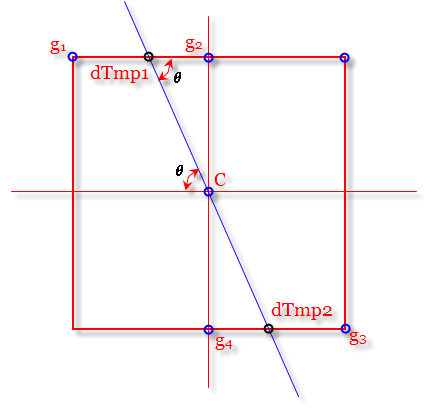
\includegraphics[width=3in]{nms2.png}
    \caption{非极大值抑制}
    \label{fig:nms2}
    \end{figure}  




\subsection{双阈值}
MATLAB中Canny算子是自动设置双阈值的。

通过统计得到边缘图的灰度直方图,然后计算得到累积直方图。用累积直方图0.7处的值作为高阈值。低阈值=高阈值*0.4。

\section{在OpenCV中}

\subsection{非极大值抑制}
OpenCV中Canny函数在实现非极大值抑制时,不进行插值,直接比较该点与其8邻域内梯度方向附近两点的梯度值大小。例如如图\ref{fig:nms1},图中黑色线表示该点的梯度方向,梯度方向在0和4区域范围内,只需与8邻域内a点和b点进行比较。同理,如果在1和5区域内,与8邻域内c点和d点进行比较……
    \begin{figure}
    \centering
    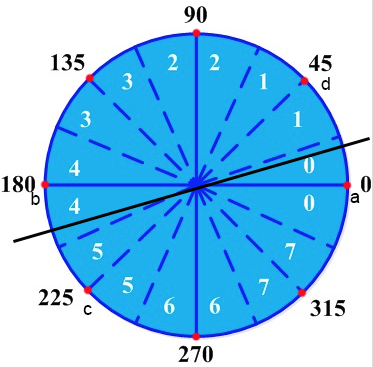
\includegraphics[width=3in]{nms1.png}
    \caption{非极大值抑制}
    \label{fig:nms1}
    \end{figure}  

\subsection{双阈值}
OpenCV中Canny函数的双阈值是人为设定的。
  \begin{lstlisting}[language=c++]
    Canny(InputArray image, OutputArray edges, double threshold1, double threshold2)
  \end{lstlisting}









%%---------------------------------------------------------------------
\end{document}
